\documentclass[11pt]{article}

\usepackage[margin=1in]{geometry}
\usepackage[T1]{fontenc}
\usepackage[utf8]{inputenc}
\usepackage{lmodern}
\usepackage{microtype}
\usepackage{amsmath,amssymb,amsthm,mathtools}
\usepackage{graphicx}
\usepackage{float}
\usepackage{placeins}
\usepackage{booktabs}
\usepackage[hypcap=false]{caption}
\usepackage{subcaption}
\setcounter{topnumber}{4}
\setcounter{totalnumber}{6}
\renewcommand{\topfraction}{0.9}
\renewcommand{\textfraction}{0.1}
\renewcommand{\floatpagefraction}{0.8}
% Top-align content on float-only pages (avoids large centred white space above tall figures).
\makeatletter
\setlength{\@fptop}{0pt}
\setlength{\@fpsep}{8pt plus 2fil}
\setlength{\@fpbot}{0pt plus 1fil}
\makeatother
\usepackage{enumitem}
\usepackage{xcolor}
\usepackage{csquotes}
\usepackage{hyperref}
\usepackage[nameinlink,noabbrev]{cleveref}

\setcounter{secnumdepth}{3}
\setcounter{tocdepth}{2}
\allowdisplaybreaks
\setlength{\parindent}{1.2em}
\setlength{\parskip}{0.15em}

% Thesis-compatible macros (from AA_Thesis / Thesis.tex)
\newcommand{\pr}[1]{{\text{Pr}\left\{#1\right\}}}
\newcommand{\mean}[1]{{\rm I}\!{\rm E}(#1)}
\newcommand{\rr}{{\bf R}}
\newcommand{\xx}{{\bf X}}
\newcommand{\xt}{{\xx_t}}
\newcommand{\yy}{{\bf Y}}
\newcommand{\yt}{{\yy_t}}
\newcommand{\ww}{{\bf W}}
\newcommand{\ddt}[1]{\frac{\mathrm{d}#1}{\mathrm{d}t}}
\newcommand{\pdx}[2]{\displaystyle\frac{\partial #1}{\partial #2}}

\theoremstyle{plain}
\newtheorem{theorem}{Theorem}[section]
\newtheorem{proposition}[theorem]{Proposition}
\newtheorem{lemma}[theorem]{Lemma}
\newtheorem{corollary}[theorem]{Corollary}

\theoremstyle{definition}
\newtheorem{definition}[theorem]{Definition}

\theoremstyle{remark}
\newtheorem{remark}[theorem]{Remark}

\hypersetup{
  colorlinks=true,
  linkcolor=blue!55!black,
  citecolor=red!55!black,
  urlcolor=blue!60!black,
  pdftitle={Introduction (Chapter 1)},
  pdfauthor={Adam Aldridge}
}

\title{Introduction}
\author{Adam Aldridge}
\date{Extracted from AA Thesis (Chapter~1)\\University of Leeds, November 2024}

\begin{document}

\maketitle
\vspace{-1.5em}

\begin{abstract}
\noindent
This chapter introduces the biological and mathematical setting of the thesis.
It motivates a stochastic treatment of early \textit{Yersinia pestis} infection,
reviews branching-process ideas used throughout, sketches the biphasic
pathogenesis of plague, and situates the basic model of viral replication (BMVR)
and bursting-versus-budding release strategies. Research questions and a roadmap
of the remaining chapters are given at the end.
\end{abstract}

\tableofcontents
\clearpage

% Opening of Chapter 1 (Introduction)

The Yersinia pestis bacterium is the causative agent of bubonic plague. Perhaps more than any other human pathogen, it has struck fear into the hearts and minds of peoples all over the world, and consciously or not lingers as a shadow in the western psyche. 

The present thesis will explore the mechanisms this bacteria employs in a human host, and the strategies it has evolved to overcome our innate immune system which possibly facilitated its historical success. 

We will paint a mathematical picture of an early stage plague infection with the aim of shedding light on the challenges faced by Yersinia pestis, and potentially the strategic advantege of its niche method.

\section{Bubonic plague}
Yersinia pestis (Y. pestis) was first identified in 1890 by Alexander Yersin. It was later attributed (and only recently confirmed with genomic data) to have caused a number of major epidemics which killed a huge proportion of the European population and went on to shape the course of western cultural development. 


In 751AD there was Justinian's plague, but the most dramatic epidemic started in 1345 and may have killed as much as 50\% of the European population \cite{belich2022world}, with this figure reaching above 80\% in some urban centres. Successive waves of infection followed this and the continent didn't fully emerge from the plight until as late as the 17th century, with the 1666 fire of London often attributed as the watershed moment.\par
There were likely earlier Y. pestis epidemics reaching far back into history beyond the scope of accurate written account, perhaps recorded only in legend and myth. Evidence for this can be seen in a recent discovery that Y. pestis emerged from its evolutionary antecedent (Yersinia pseudotuberculosis) around 6000 years ago during what would have been a period of human population expansion driven by the development of agriculture. We may hypothesise that it was this excess supply of replicative means which provided the raw material for evolution. Facilitating a shift in phenotypes over the saddle into a new local optima. This representing the niche pathogenesis observed today in Y. pestis.

\section{Stochastic modelling}

Generally, at the outset of an infection, a relatively small number of colony forming units (bacteria or virus) will enter the body. 
Be it during inhalation into the respiratory system, through the skin with an insect's bite, or via ingestion, those initial pathogenic particles will be critical in determining the fate of the infection's success. 

The founding population will either be depleted to extinction, or expand to a capacity where its growth becomes established and requires a more targeted effort of the immune system to deal with. Whether they succeed in surviving beyond the first few hours of infection will depend on causes of a chance nature; encounters with cells and other immune factors that are subject to the randomness of Brownian motion.  


Stochastic effects play a more significant role in a population which is small. Because as the count of individuals increases, the dynamics of their overall growth and decline will become increasingly subject to the law of large numbers, and the expected fate of particular bacteria becomes telling of the group's trajectory. 

For this reason, because we are interested in the early stages of a Yersinia Pestis infection, it will be important to use stochastic models in our analysis.

\section{Branching}

Branching is one of the most fundamental patterns of behaviour observable in living systems. It is a basic means for the ordered structures of living entities to expand indefinitely in response to resource supply. Dividing one individual into two allows biomass and hence dissipative potential to increase without paying the cost required to increase agent complexity.\par

At the most basic level, replication of DNA molecules makes up the foundational component of all biological life. It is the maintenance and development of information, held up and carried forward against all odds of decay.\par

Understanding branching from a mathematical perspective has been a topic of probability theory since the end of the 19th century. Darwin's cousin, Francis Galton sought to understand the persistence of family names over generations. For this, with Henry Watson, he employed what would come to be known as the Galton Watson process  \cite{watson1875probability}. It's a discrete time stochastic process in which individuals either die or leave some number of offspring at each generation, fate being dictated by defined probabilities.\par 

It wasn't until the 1920s that continuous time models of branching were developed. In 1924, George Undy Yule published a paper in response to a book on evolution. The book was called ``Age and area'' and sought to understand the relationship between the number of species in a living genus and the area over which it spans. The paper  \cite{yule1925ii}, introduced what would become known as the Yule process. This was the first continuous time model of branching. Individuals only replicate, and do so with some probability during an interval of time:
$$\pr{\xx_{\Delta t + t}  = \xt + 1 \;\; | \;\; \xt} = \beta \xt \Delta t + o(\Delta t).$$
As the interval is taken in the limit, $\Delta t\to 0$, the probability that more than one replication takes place becomes infinitesimal. The fact that any of the $\xt$ present individuals can reproduce is encoded by the proportionality of the birth rate $\beta \xt$.\par This model, applied equally well to bacterial replication as to the emergence of species is also known as the standard birth process. Introducing death events, we get the standard birth-death process:

$$\pr{\xx_{\Delta t + t}  = \xt + 1 \;\; | \;\; \xt} = \beta \xt \Delta t + o(\Delta t)$$
$$\pr{\xx_{\Delta t + t}  = \xt - 1 \;\; | \;\; \xt} = \mu \xt \Delta t + o(\Delta t),$$

\noindent
which now has a universally accessible absorbing state at 0 representing extinction. Much of the work presented in this thesis surrounds our analysis of a further modification to this birth-death process. An additional ``catastrophe event'' is introduced whereby a sudden transition can take place from any non-zero count either to 0 or a separate ``rupture state'' (as per choice of definition).

$$\pr{\xx_{\Delta t + t}  = \xt + 1 \;\; | \;\; \xt} = \beta \xt \Delta t + o(\Delta t)$$
$$\pr{\xx_{\Delta t + t}  = \xt - 1 \;\; | \;\; \xt} = \mu \xt \Delta t + o(\Delta t)$$
$$\pr{\xx_{\Delta t + t}  = R \;\; | \;\; \xt} = \delta \xt \Delta t + o(\Delta t).$$

\noindent
In our case this is to represent the possibility of any resident bacteria within a white blood cell to trigger a bursting event in which the walls of the macrophage disintegrate and the pathogenic contents are simultaneously released.

\section{Early phase Yersinia Pestis infection}

Y. pestis differs from its evolutionary antecedent, Y. pseudotuberculosis in a few ways but one stands out. Y. pestis exhibits two phases in its pathogenesis of mammalian hosts. In the first, the bacteria are readily absorbed by host leukocytes via phagocytosis (white blood cells, mainly macrophages and neutrophils). Within macrophages especially, the bacteria replicates in relative shelter and secrecy from patrolling immune agents.\par
In the second phase, after a switching period, they prevent this absorption by a combination of resistance and neutralisation. This is probably to avoid the more aggressive neutrophils which arrive at the infected area after a period, with recruitment following pathogen detection. This work explores the mathematical implications of this switching in an attempt to quantify the significance of the strategy's evolutionary advantage.\par 


This shift in phase of the incident bacteria occurs in response to sensing the warmer ambient temperature of a mammalian host. At a cooler temperature inside a flee, the bacteria remains in its first phase. Then after the flea bites its host, injected bacteria will after some delay shift behaviour to the second phase. The key difference acquired is resistance to phagocytosis. At the outset of invasion, colony forming units will be absorbed (phagocytosed) by host macrophages. With evolved resistance to their toxins, Y. pestis bacteria use this intracellular refuge as a temporary home to replicate and bolster numbers against challenges to come. The first mounted attack of the innate immune system is neutrophils. Summoned by various cytokines, they arrive on the scene in numbers, passing through the walls of blood vessels to the extracellular matrix in which the infection is beginning to take hold. After some time, an infected macrophage will rupture and its resident bacterial population will disperse into the extracellular matrix. Those Y. pestis bacteria which have undergone the transition to the second phase are characterised by being resistant to further phagocytosis.  Figure \ref{fig:two_columns_six_image} illustrates the dynamics. 


\begin{figure}[h!]
    \centering
    % First row of two images
    \begin{subfigure}{0.48\textwidth}
        \centering
        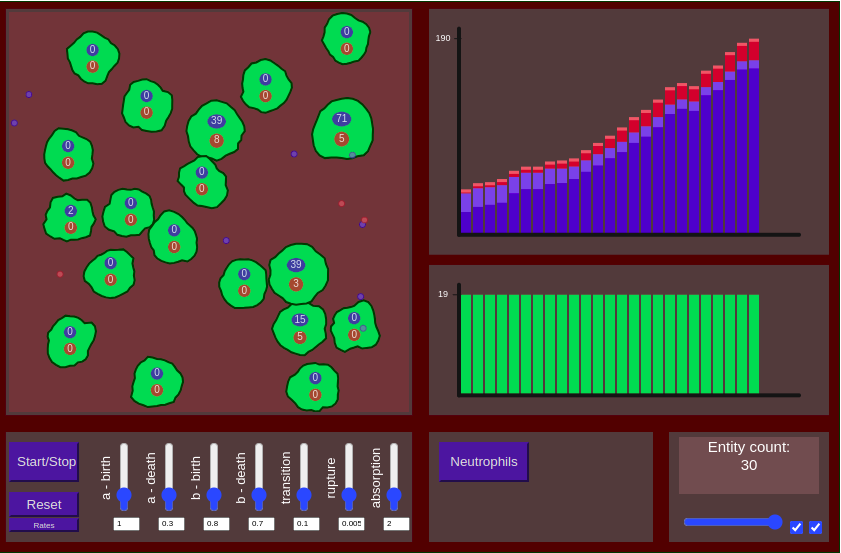
\includegraphics[width=\textwidth]{figures/fig_yp_schematic/web1}
    \end{subfigure}
    \hspace{\fill}
    \begin{subfigure}{0.48\textwidth}
        \centering
        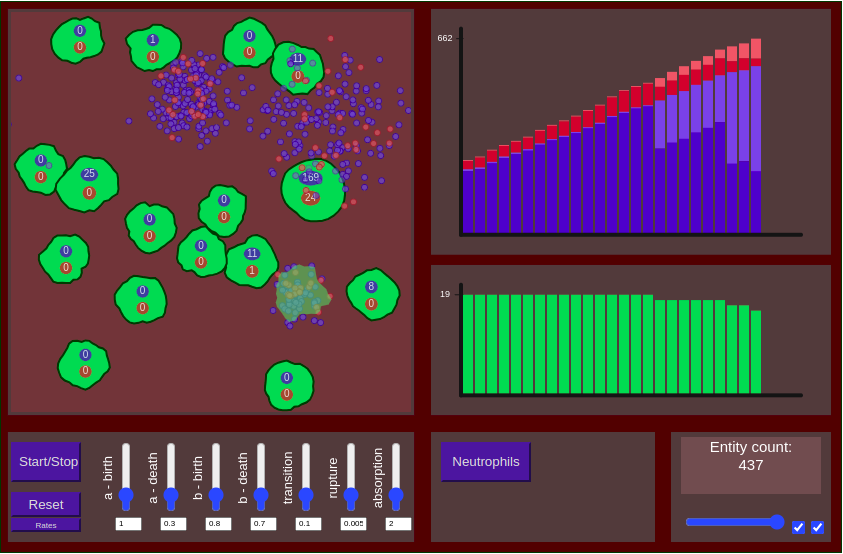
\includegraphics[width=\textwidth]{figures/fig_yp_schematic/web2}
    \end{subfigure}

\caption*{Bacterial replication takes place within macrophage.  Some phase transitions occur.}
    \vspace{0.5em} % Small vertical space between rows

    % Second row of two images
    \begin{subfigure}{0.48\textwidth}
        \centering
        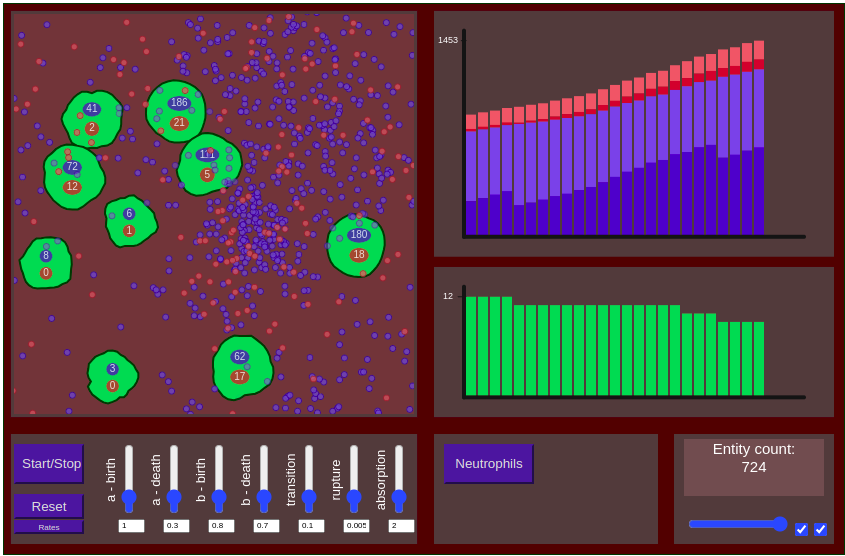
\includegraphics[width=\textwidth]{figures/fig_yp_schematic/web3}
    \end{subfigure}
    \hspace{\fill}
    \begin{subfigure}{0.48\textwidth}
        \centering
        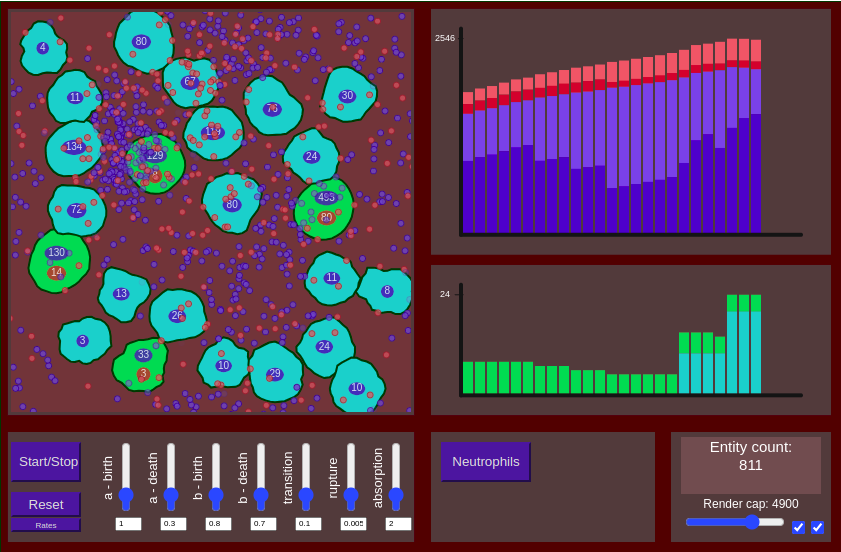
\includegraphics[width=\textwidth]{figures/fig_yp_schematic/web4}
    \end{subfigure}

\caption*{Macrophage bursting,  more transitions to the second phase (red particles).  Neutrophils arrive.}
    \vspace{0.5em} % Small vertical space between rows

    % Third row of two images
    \begin{subfigure}{0.48\textwidth}
        \centering
        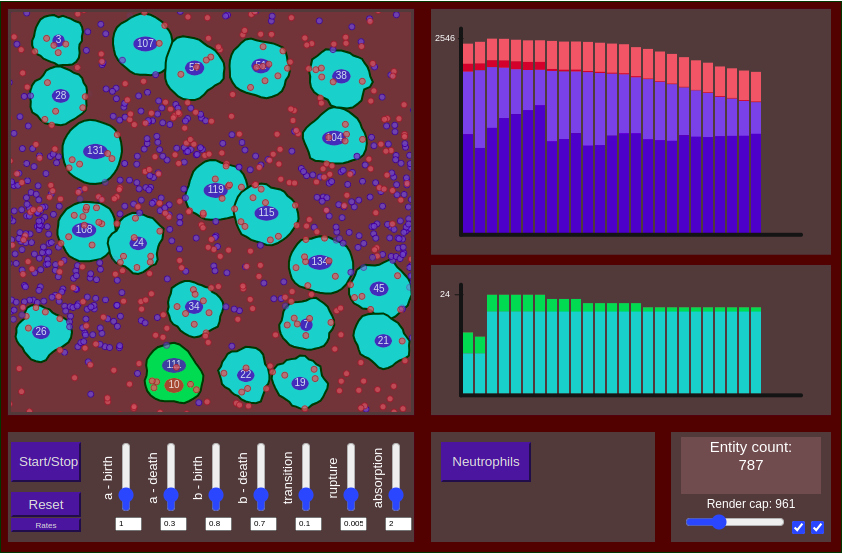
\includegraphics[width=\textwidth]{figures/fig_yp_schematic/web5}
    \end{subfigure}
    \hspace{\fill}
    \begin{subfigure}{0.48\textwidth}
        \centering
        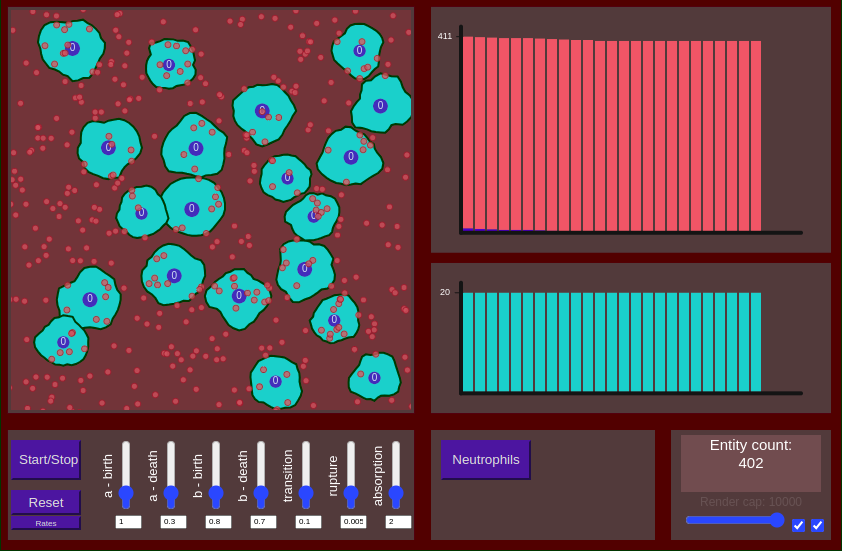
\includegraphics[width=\textwidth]{figures/fig_yp_schematic/web6}
    \end{subfigure}

    % Single caption for all images
\caption*{Neutrophils phagocytose and eliminate remaining phase one leaving Y. pestis as a primarily extracellular infection.}
    \caption{A schematic representation.}
    \label{fig:two_columns_six_image}
\end{figure}

\section{HIV and the basic model of viral replication}
In the 1980s there was a major global HIV epidemic. This was terrible, killing around 40 million people over the decade, but it had the positive side effect of inducing a flurry of research into HIV pathogenesis and viral dynamics more generally. By the early 1990s progress was being made with the development of effective mathematical models describing within host viral replication.\par
Principal among these was what became known as the Basic Model of Viral Replication (BMVR) \cite{mclean1993balance}, which emerged from the fray of model diversity following the period of substantial experimentation. Its basic assumption was quite simple: there are three agent types

\begin{itemize}
\item \textbf{Susceptible cells: $S$} 

Host cells produced with a constant influx of rate $\lambda$, removed as they become infected by individual virions with a rate $\beta$.

\item \textbf{Free virions: $V$}

Produced at a constant rate, $p$, by each infected cell, and also cleared with rate $c$.

\item \textbf{Infected cells: $I$}

A single free virion coming into contact with a susceptible cell is sufficient to convert it into an infected cell. Naturally, this uses up the virion and removes one succeptible cell from $S$. Infected cells then produce new free virions at a constant rate, not accounting for the likely reality that a higher intracellular load might cause a cell to be more productive. Though some models do include a lag period between the time a cell is infected and when it begins to produce virions.\par
They are also removed by cell death with rate $\delta$.
\end{itemize}

\noindent
The equations are as follows

\begin{align*}
\ddt{S} & = \lambda - \beta SI\\
\ddt{I} & = \beta SI - \delta I\\
\ddt{V}& = p I - c V.
\end{align*}

\noindent
In some cases, the model is simplified by taking the number of susceptible cells as a constant, $T$. This represents the situation in which there is a large availability of cells to infect such that their depletion is not a significant driver of the overall dynamics. With this simplifying assumption, the equations become,

\begin{align*}
\ddt{I} & = \beta TI - \delta I\\
\ddt{V}& = p I - c V.
\end{align*}

\noindent
To be clear, this rests on the assumption that virions are produced by cells one by one at a constant release rate.


\subsubsection*{New research into HIV viral release}

In 2018, an experiment was done at Los Alamos \cite{hataye2019principles} with the intention of quantifying the release dynamics of HIV virions from infected cells. A tray of 32 small ``wells'' were each filled with some liquid each containing exactly one cell infected by HIV. Then over a period of days, viral counts were measured from the liquid of every well at intervals of one hour.\par

If the assumption of the BMVR were correct, we would expect to see something approximating a Poisson process in each well, with roughly the same count recorded in all of the wells at each interval. What was actually observed was very different: huge variation between wells, and the production rates were not at all constant. Instead, a high degree of intermittency was recorded. Cells remaining completely inactive for successive intervals, then occasionally releasing a substantial number of virions, seemingly all at once. \par

Clearly, this challenges the standard assumption of constant-rate budding. It also raises a speculative question: Could this commonly held belief about viral release have been to some extent patronised by widespread use of the modelling assumption? We'll probably never know, but it's curious to consider.\par

\subsubsection*{So what?}
In any case, the observation is interesting and it begs the question: why? There will be some reason HIV has evolved to use this quasi-bursting procedure. Perhaps it is simply more convenient for release to take place in floods. Passage through the cell wall requires an opening, and it surely makes sense to only induce this periodically; avoiding both unwanted leakage of cellular components and ingress of extracellular debris.\par 

But perhaps there is also some general advantage to be gained by virions being released in large cohorts like this. It could be that locally deletable immune factors are flooded and overcome by the sudden outflux of enemy agents. A paper by N. Komavora \cite{komarova2007viral} presented this idea of a so called ``flooding'' advantage. She used the analogy of a criminal gang trying to escape their trap house which is surrounded by police: ``If we all run out at once, maybe some of us will get away in the confusion''.\par 

Analysis of pathogen release strategies and their potential makes up the topic of chapter 6, with attention paid to the spectrum between budding release, and complete cell bursting.\par

Back on the topic of the BMVR and its potentially flawed assumption, in chapter 4 we propose a possible modification to the viral release term, $pI$, in an attempt to account for intracellular dynamics consistent with the birth death catastrophe process.

\section{Pathogenic release strategies.} 

With both viral and bacterial particles being very small, it has historically been extremely challenging to make good observations of their behaviour. Progress is taking place, and in the last couple of decades, we have been able to observe individual bacteria through the course of an intracellular infection. For example, Dstl (Defence science technology laboratory) has been able to record videos of a macrophage bursting to release on the order of 100 Francisella Tularensis bacteria. Through the induction of bacterial luminescence, each individual pathogenic particle can be visually isolated and counted.\par
Francisella Tularensis and Y. Pestis are similar in size, each around 0.5 micrometers (Y. pestis being marginally larger). But viruses are generally about an order of magnitude smaller than bacteria, with HIV being approximately 100 nanometres. They are hence somewhat more elusive to visualisation and counting.\par 


\subsubsection*{Bursting}
Both Francisella Tularensis and Yersinia Pestis multiply within macrophages becfore causing the cell to lyse, releasing their pathogenic cohort for further replicative endevours. The case of Y. Pestis is slightly more complicated with a biphsaic switching; a change from intracellular to extracellular replication (more on that later). But generally, these strategies which involve a complete release in combination with the death of the cell are reffered to as bursting pathogenesis.

\subsubsection*{Budding}

As described above, budding release refers to the situation where an infected cell outputs new virions at a constant rate. Models of viral replication generally take this as an assumption and it has become a commonly held belief that this is how viral release takes place. 


\subsubsection*{Something in between?}

The recent work experimenting HIV release reveals that the story may not be so simple as was previously assumed. That in cases of non-lytic virulence there may be various strategies we are not fully aware of. Another example of something in between bursting and budding is release by extracellular vesicles (EVs). Amongst viruses that leave the cell non-lytically, there is a subdivision to be made into those which produce and assemble their own protein shell to harbour genetic material, and those which exploit the cell membrane to produce a lipid container. Of this second group, it has been known for a while that in some cases, multiple individual viruses get contained and released in one ex-membrane capsule. These are reffered to as extracellular vessicles \cite{kerviel2021new}, \cite{buzas2023roles}. They present another potential coplexity to the story of viral release.

\section{Research questions}

There are four key areas of focus that this research seeks to address. The first two are questions into the nature of biological process:

\begin{itemize}
\item  \textbf{Why did Y. pestis evolve a biphasic pathogenesis in humans?} 
Switching from pro-phagocytosis to an antiphagocytosis strategy seems to be crucial to the overall pathogenesis of Y. Pestis.  There is a simple argument based on the net proliferability both before and after neutrophils arrive on the scene of infection (see conclusion).  Also,  we could assume that Y. pestis replication is only slightly supercritical.  And it can be easily demonstrated that near critical branching process become drastically less likely to die out when the initial count is increased by even a few colony forming units.  If we see the initial within macrophage replication as setting up an initial population,  this effect offers further explanatory potential. 


\item \textbf{Is there a general advantage to "bursting" style transfer in successive intracellular infection methods?}
Natalie Komavora proposed that there could be a "flooding advantage" to bursting style pathogenesis.  That is,  bacteria or virus exiting their host infected cells all at once in large groups rather than one at a time or in dribs and drabs. Chapter 7 explores gives further mathematical support to this theory and discuses the conditions under which it might prove effective.
\end{itemize} 

\noindent
The second two are areas in which we tried to construct new models to describe particular dynamics:

\begin{itemize}
\item \textbf{A potential update to the standard BMVR model of viral replication to incorporate intracellular dynamics.}
Based on our analysis of the birth death catastrophe process, there is the possibility that one of the results could be encorporated into a rate of the BMVR.

\item \textbf{Efforts to describe variable rates of evolution with Markov chains}\par
The standard birth-death process has been used for decades to model the emergence of species over geological time periods. It may however be criticised for being consistent with the outdated doctrine of progressive gradualism. This states that evolutionary change is constant and happens gradually. In the 1970s,  S. J Gould proposed the counter theory of punctuated equilibria: evolution taking place rapidly over proportionally short periods which are intervened by longer times of relative morphological stasis.\par
There is also the controversial question of why large clades (containing many species) appear to generally have experienced an initial period of substantial diversification. Some attribute this observation to a statistical consequence of standard birth-death dynamics (push of the past, and pull of the present).\par
This work presents two models which seek to challenge this argument, and give mathematical basis to the punctuated equalibria theoretical paradigm. Notably, there is potential significance here in understanding the emergence of Y. Pestis.


\end{itemize}

\section{How the content is divided amongst the chapters}

Broadly, the thesis can be divided into three main parts: Introductions,  analytical results in relation to the Birth Death Catastrophe process,  and models of resulting from my curiosity.  Including this introduction and the conclusion,  these parts are divided amongst 8 chapters.  Below is a summary of the content and message of each.


\subsubsection{Chapter 2: Mathematical context}


Much of the work presented in this thesis surrounds topics of stochastic process theory,  and specifically branching processes.  Both continuous time and discrete time branching processes are examples of Markov chains exhibiting the Markov property: The probability of what happens next depends only on the current state of the system,   not on any past events;
\[
P(\xx_{t+1} = x_{t+1} \mid \xx_t = x_t, \xx_{t-1} = x_{t-1}, \ldots, \xx_0 = x_0) = P(\xx_{t+1} = x_{t+1} \mid \xx_t = x_t).
\] 
Continuous and discrete time Markov chains differ in their methods of analysis.  For example,  the fixation probabilities of discrete time processes can be understood using first step analysis which considers the single-step possible moves and their probabilities.  Continuous time chains on the other hand can be dealt with using the forward Kolmogorov Equation.  It is worth noting that continuous time chains can be "embedded" into discrete time versions by considering the probability distribution of \textit{next} events.  But when it comes to branching processes,  this fact shouldn't give the false impression that the two types of process are somehow identical in their dynamics,  just on modified time axes. Discrete time branching proceses differs fundamentally in that every individual either replicates or dies at once in each time step.  In the continuous time birth death process,  only single jumps up or down are possible at each move.  And this difference means there isn't a clear analyitical transformation between the two types of model.\par
It should be noted that we will only be dealing with discrete state space processes (jump chains).  Continuous state space models are also of interest, but the application to cellular replication nautrally lends itself to models with countable units. 
\vspace{10pt}

\noindent
One of the most important aspects of branching processes is their net replacement. This has slightly different interpretations in discrete and continuous time branching but esentially means the same thing.  It is the rate of change of the expected process count.  In discrete time: the expected number of offspring produced by a single individual in its lifetime.  
$$\mean{Z} = 2 p + 0(1-p) = 2p$$  
where p is the probability of an individual to replicate rather than die (wp $1-p$), and $Z$ is the number of offspring left by the one individual. \par 
In continuous time,  rate of population expansion,
$$\ddt{\mean{\xt}} = (\beta - \mu) \mean{\xt},$$
is quantified by $\beta - \mu$,  the net replication rate. 
In each case,  whether this number ($2p$ or $\beta - \mu$) is larger or less than 1 is of great signigicance. 


\begin{itemize}
\item When $2p$ or $\beta - \mu$ greater than 1,  the process is caled supercritical.  (see figure 1.2)
\begin{figure}[h!]
\centering
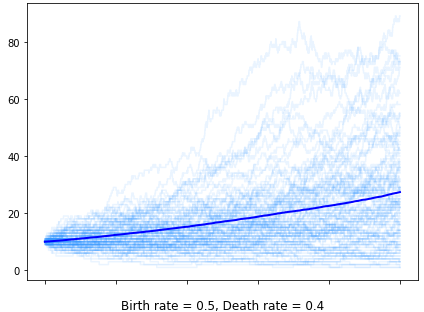
\includegraphics[width = 0.55\textwidth]{figures/fig_bd_regimes/BD54}
\caption{Supercritical birth death in continuous time.  In this and the following two figures, a large numer of individual realisations are shown in light blue, and their average is drawn in dark blue.  In each case, the sample mean shown forms a good approximation of the analytical mean.}
\label{im1}
\end{figure}
Some realisations die out, the rest continue rising towards infinity in an increasingly redictable exponential fashion. 
\end{itemize}


\begin{itemize}
\item When $2p$ or $\beta - \mu$ less than 1,  subcritical.  
\begin{figure}[h!]
\centering
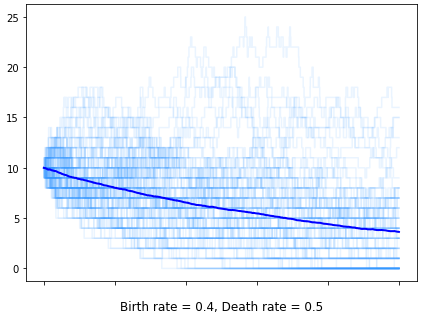
\includegraphics[width = 0.55\textwidth]{figures/fig_bd_regimes/BD45}
\caption*{Subcritical}
\end{figure}

All subcritical realisations are destined to die,  fixating at 0.


\end{itemize}


\begin{itemize}

\item And when $2p$ or $\beta - \mu$ is equal to 1,  the process is reffered to as critical.   

\begin{figure}[h!]
\centering
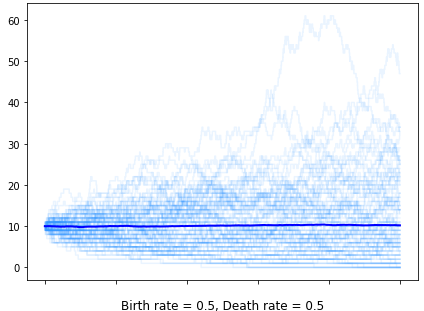
\includegraphics[width = 0.55\textwidth]{figures/fig_bd_regimes/BDpoint55}
\caption*{Critical}
\end{figure}

Line in the subcritical case, all critical realisations are destined to die out, but curiously, the expect time in which then do this is infinite.  A single process could possibly last for a very long time,  never fixating. 

\end{itemize}


\subsubsection{Chapter 3: Birth death catastrophe model -- main results}

This chapter introduces the Birth Death Catastrophe (BDC) process and outlines a series of results asociated with in. \par


\noindent
Around the 1980s, work was being done into growth models that incorporated stochastic declines (shocks). Out
of this came the the birth death catastrophe model as we know it \cite{cairns2004extinction}\cite{brockwell1985extinction} \cite{brockwell1982birth} \cite{dori2018family}.  An extension of the standard birth death
process, but where from every state apart from 0, a catastrophe event can take place, either causing a transition
to 0, or a special catastrophe state. Similar to birth and death events, this catastrophe state can be initiated by
any of the individual units, and so occurs with a rate proportional to the population size. We were interested
in this model for its potential application in modelling the development of an infection within cells that burst.
And more broadly, infections that spread amongst multiple cells.
Here the BDC model is defined and some key equations are introduced which describe the mean and variances
of the process. Some of the results have been found by others before, but we also have a few which extend beyond
the current literature. For example, we have a formula for the second moment of the process count in terms of the non-rupture probability. This, along with the process variance we found by solving a series of four ordinary differential equations.\par

Some attention is given to limiting conditional distributions. That is the behaviour of the process count assuming that by some late time fixation has not yet occurred.  We show that in some cases, quasi-stationarity is exhibited and we quantify the quasi-stationary mean as a function of rate parameters for replication and rupture.


\subsubsection{Chapter 4: Birth death catastrophe model -- additonal results}

This chapter extends the pervios one with more results,  especially those associated with state probabilities which are obtained from the forward Kolmogorov equation with the method of characteristics. 


\subsubsection{Chapter 5: Birth death catastrophe process -- modifications}

Here we explore the analytical possibilities of two modified BDC processes
\begin{itemize}
\item $\mathbf{N = 2}$ \textbf{sucessive imediate transfer}. We were generally interested in producing some kind of model which captured the dynamics of between-cell transfer and growth.  Moving in this direction,  we spent some time developing results in relation to the successive BDC process whereby a second process begins at the rupture of the first.  The anaysis didn't lead to exactly what we were looking for, but we found some distributions along the way,  and the work ultimately went on to lay the groundwork for the "fixed removal" model of chapter 6.   


\item \textbf{Two type}.  In 2011,  Antal and Krapivsky \cite{antal2011exact} published an exact solution to the two type continuouts time birth death process with one way mutation.  We were able to use their particular method, with some changes of variables,  to obtain the equivalent result for the two type BDC process.  This section simply outlines the process by which the result can be found. 


\end{itemize}


\subsubsection{Chapter 6: Bursting-budding comparrison}


Work has been done by others \cite{komarova2007viral} \cite{yuan2011stochastic} \cite{pearson2011stochastic} \cite{capistran2018extracellular} comparing the fundamental dynamical differences between budding and bursting style pathogenesis.  N. Komavora, for example proposed a potential advantage to busrting due to a flooding effect.  This chapter explores the significance of release counts when considering successive infiltration models.  That is, where pathogens go from one infected cell to another. \par
Each of the parts of this chapter consider he importance of locally depletable immune factors.  With only a finite supply of chalenges,  there is a sort of saftey in numbers effect.


\noindent
\textbf{Replicator suppressor}
This part considers the intracelllular environment in which there are toxin containing granules such as there are in macrophages and neutrophils.  Similar to a predetor pery model,  there are two individual types: replicators (pahogenic particles) and suppressors (granules).  It is clearly demonstratable that a larger incident population of replicators will have disproportonatly beter odds of survival and persistence in this case as more bacteria will be available to deplete the present immuno reserves. 


\noindent
\textbf{Fixed removal}
Moving from the intracellular to the extracellular environment. This part considers the question of how many released pathogenic particles manage to reach their next host.  In the extracellular medium between host cells there are a number of immune chalenges that the pathogens have to face. \par
For example,  complement proteins, which puncture bacterial cells deemed to be invaders,  and host bacteriophages which are viruses living in simbiosis with the organisms that may serve to kill forein agents. \par
The assumption is that these immune factors are locally depletable and that a larger group release of pathogens will somehow cause a flooding effect analogous to the one proposed by N. Komavora. 


\subsubsection{Chapter 7: Variability in evolution}
No topic has seduced and captivated my curiosity more than the question of what life is,  how it evolves,  and whether we can determine general underlying dynamics which uncover aspects fundamental to the reality of rise,  change,  and decay of living agencies. \par

Evolution into species, harbours a yet unsolved mystery to science.  We do know a lot.  For example,  vast efforts have been made in the last 5 decades into uncovering the microbiological mechanisms which underpin the replication and usage of DNA. \par


With regards to a big picture view,  progress is being made \cite{sharma2023assembly},  but we are yet to produce a widely taught and accepted description of what life is and how it changes which is consistent with concepts of neg-entropy production and thermodynamics more generally at the micro and macro scales. \par

But the hum and the buzz has been around for a while now,  and perhaps the writing is even on the wall as to how a water-tight conception might unfold.

Unfortunately,  this thesis does not have the answer.  Not only am I considerably under-qualified for the task,  but this project was supposed to be about Yersinia Pestis,  and it largely is.  Of course,  Y.  pestis bacteria is one of the most acute examples of a living dissipative structure.  \par

\vspace{10pt} 


\noindent
 Mostly before the PhD and in the first year,  I read a few books which went on to change the way I thought about science,  philosophy,  and particularly the topic of evolution.  Most significantly: 


\begin{itemize}
\item \textbf{Order out of chaos,  Mans new dialogue with nature --  Ilya Prigogine and Isabelle Stengers,  1984}
Outlines the theory of dissipative structures -- chaotic order formations which take place as local reductions in entropy in the as a means of dissipation in the context of a wider increase in entropy consistent with the second law \cite{prigogine2018order}.

\item \textbf{What is life -- Erwin Schrödinger, 1944}
Frames the problem of understanding what life is in the context of energy gradients,  neg-entropy and the laws of thermodynamics \cite{schrodinger1946life}.   

\item \textbf{Chance and necessity -- Jacques Monod, 1970}
Overviews the (at the time) new understanding of DNA molecular biology and mechanisms of replication and transcription \cite{monod1974chance}.  Then explores the concept of teleology and what it means for living objects, made of mere chemistry, to have volition. \par 
Outlines animism and vitalistic schools of thought and belief.

\item \textbf{The genetical theory of natural selection -- Ronald Fisher, 1930}
Covers the topic of evolution broardly from a mathematical perspective. Then goes on to discuss the implications of birth rates being different among sectors of society.  Also the rise and fall of civilisations. \cite{fisher1929genetical}. 

\item \textbf{Wonderful life -- Stephen J Gould, 1990}
All about the Cambrian explosion,  a geologically instantaneous period of a few million years in which great diversification of species took place.  Contrasting the previous Ediaceran fauna of docile wandering discs of the sea floor, all of a suden, there were a vast array of segmented athropodic forms.  Displaying arms, legs, eyes, mouths and claws;  eating one another and josstling for survival in what must have been a tropical tempo of savage egoisms \cite{gould1989wonderful}. 

\item \textbf{Beyond good and evil -- Friedrich Nietzsche}
Covers a wide range of topics surrounding, from the historical development of moralities to the emergence of species in relation to environmental conditions and suspended potential within a population.  \cite{nietzsche2013beyond}

\item \textbf{(Some of) On the origin of species -- Charled Darwin, 1859}
Needs no introduction.  Hard to read though with the old timey langauge style! Mostly interested in what he said of rate of variation in cases of domesticated animals.  \cite{darwin1859origin} 
\end{itemize}


They drew my attention to fact that the rate of evolution and divergence into species,  among other things,  is driven by a combination of selective pressures and energy availability.  For example,  the presence of competing species and how much food is readily available for a given population in its ecosystem.  It seems that these two factors make up a kind of push-pull tension,  simultaneously holding a group together with the necessity to conform so as to be strong in the face of competition for survival; whilst constantly pulling it apart with the ravenous impulse of variation which is a natural component of living matter as consistent with the second law of entropy increase. \par

Nietzsche writes about this sort of dynamic in ``Beyond good and evil" section 262:

\begin{quotation}
\noindent
"A species arises, a type becomes fixed and strong through protracted struggle against essentially constant unfavourable conditions. Conversely, one knows from the experience of breeders that species which receive plentiful nourishment and an excess of care and protection soon tend very strongly produce variation of their type and are rich in marvels and monstrosities"
\end{quotation}

\noindent
Sexual selection also offers a mystery in this space.  It seems to both macroscopically bring a population together through mixing of traits whilst also (microscopically) introducing disorder into genomes crossed over.  I won't attempt to make heads or tails of this apparently confusing juxtaposition.  Maybe someone else has and perhaps it isn't as confusing as it may appear. \par 

\vspace{10pt}

\noindent
 
\noindent
But my suspicion is that there is a underlying dynamic to articulate.  That there is a building of tension,  and release at the advent of more favourable circumstances.  And that this takes place in a cyclic fashion across multiple domains. \par

That this release is as it were more dissipative,  and during it,  when there is a greater fanning out of forms,  that this is an example of a dissipative structure which produces a chaotic formation of complex order in the form of bifurcating species and forms.  Sort of as in fluid turbulence bifurcating fluid trajectories create a chaotic dissipation of heat through friction.  The analogy is albeit more artistic than scientific,  but fun to think about! \par
If we consider the example of planar flow around a circle,  there is here this property of a cyclic to and fro -- flow speeding up followed by turbulence shedding,  low pressure and repetition. 

\vspace{8pt}
\hrule 
\vspace{8pt}
\noindent
\textbf{Bit of an aside:} I can't help but be interested in the possibility that this sort of speculated dynamic could be used to apocryphally explain cultural trends in societies.  One potential example is the apparent trend for strict conservative values to become prevalent after a period of substantial economic and cultural dynamism which ultimately brought about liberal tolerance.\par

It could be hypothesised that this has happened at least twice before in history: In Iraq and the middle east more broadly after its golden age of expansion in the first few centuries of the second millennium, and also in Sumatra and Java of Indonesia in the 16th century after the eventual decline of the Hindu kingdoms.  (The Hindu court culture was all pushed to Bali where it survived -- see David Attenborough's 1969 documentary "The miracle of Bali",  It's not particularly relevant to the point,  but definitely worth a watch anyway).  Note: I only discovered the theorey of anacyclosis \cite{podes1991polybius} after writing this, but there appears to be some similarity. 

\begin{figure}[h!]
\centering
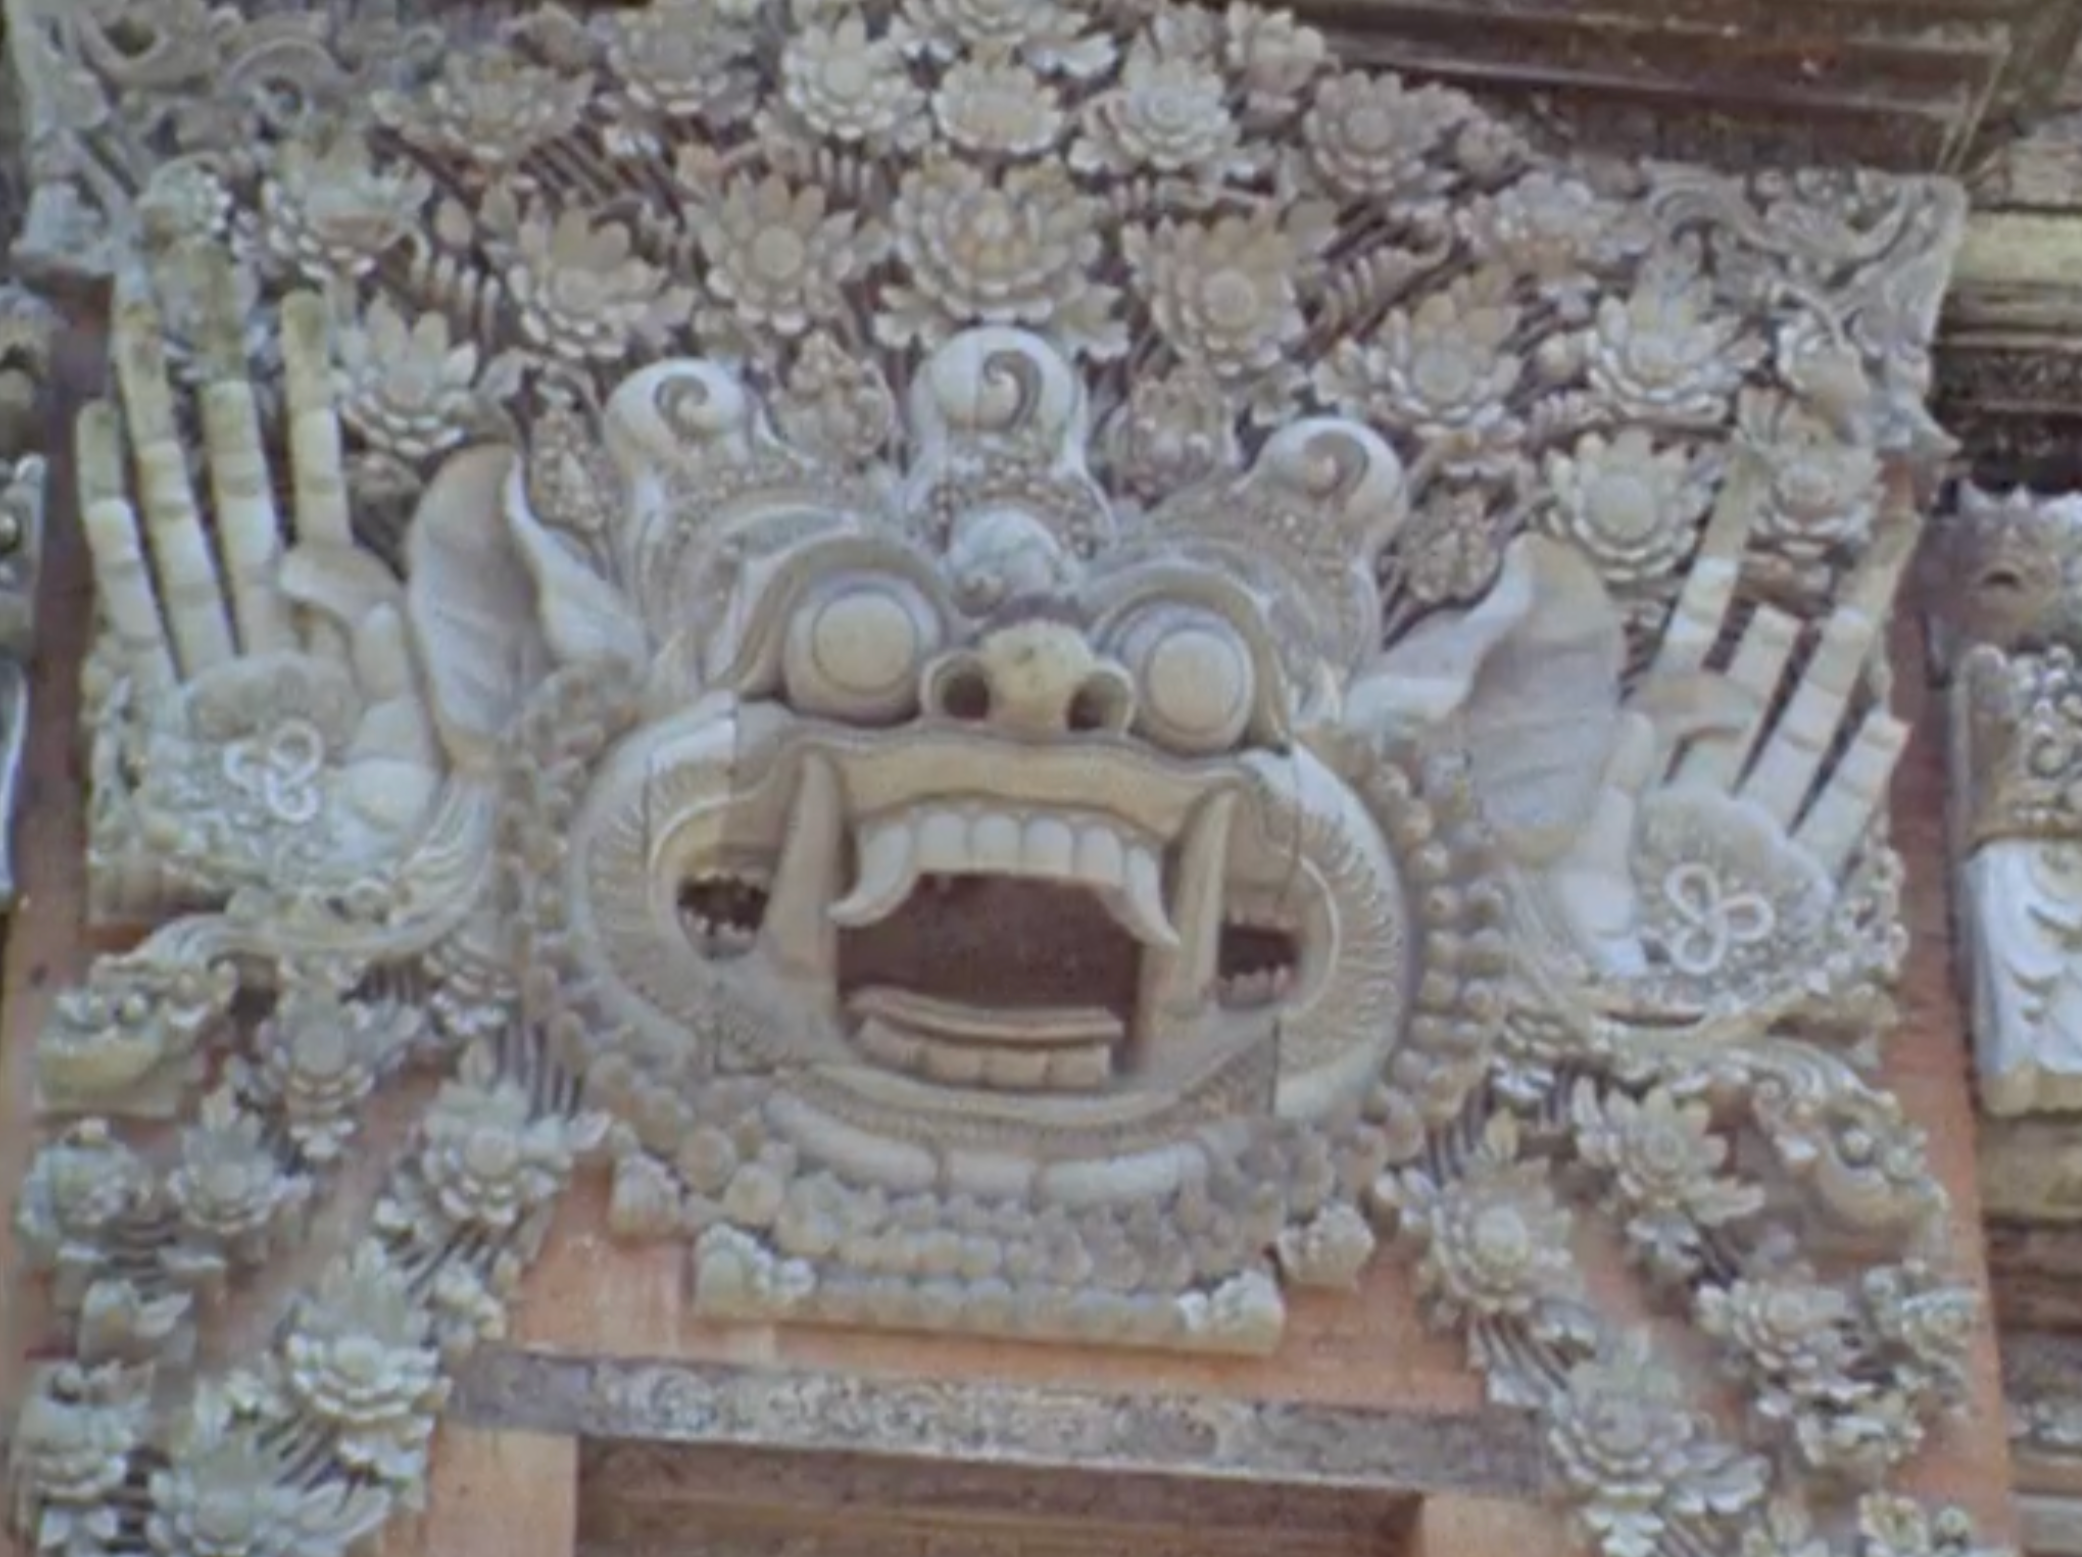
\includegraphics[width = 0.8\textwidth]{figures/fig_bali/bali}
\caption*{A carved image on the wall of a Balinese temple. Interesting how the face appears threatening, whilst also being surrounded by an emination of flowers. }
\end{figure}

\vspace{8pt}
\hrule
\vspace{8pt}

The content of this chapter is divided into two key sections accompanied by some more vapid topics of a more divergent nature.  Here is outlined the two key parts: 

\begin{itemize}
\item  \textbf{ Logistic speciation} In the spirit of Yule's 1924 paper and other more recent work with birth death processes, \cite{nee1994extinction} a continuous time Markov chain is formulated to model the production of species within a genus.  This model differs from the standard birth death process by having an inhomogeneous origination rate.  That is, the rate at which new species emerge is a function of time 
$$\beta(N(t)) $$
which is based on the relative availability of resources for a genus population which is expanding into a domain. The logistic model is used to describe the size of the population $N(t)$ in relation to its carrying capacity,  $K$  and this relative difference is taken to form the basis of the origination rate $\beta$. 


\item \textbf{ Pimentel fly model (cyclic competitive exclusion)}
"The ecological theatre and the evolutionary play" (G.  E.  Hutchinson) contains a summary of an experiment done by someone called Pimentel in the 50s.  It's purpose was to challenge the theory of competitive exclusion which states that two species can not simultaneously occupy the same niche.  It showed that an oscillation can arise when two species of fly occupy the same space provided that travel through the space is slowed by a series of compartments within the container.  This being because when one species gets pushed to near extinction,  it evolves more in response to infraspecific competitive interactions than those interspecific interactions with members of its group. \par 
This part of the chapter is about a model of these observed dynamics.\par
I also propose an addition to this model which aims to mirror the dynamic talked about in the Nietzsche quote (speciation being more prevalent when the species is the dominant of the two). 


\item \textbf{Allegorical model of rise run ruin and rejuvenation}
This is a model of one of the more vapid areas of this chapter.  The concept includes a quantity aiming to quantify potential (or vitality) in the system. This quantity,  $N(t)$ being high drives the emergence of species $\xt$.  But then, high $\xt$ count has the effect of reducing the potential.  Eventually as the quantity of allowance of "potential" per species $N/\xt$ becomes particularly low (its inverse being high), the rate of catastrophe increases to the point of certain collapse,  whereby $\xt$ declines suddenly to 0.  Subject then only to Poisson revival.  \par 

This is set up with the aim of representing something like the cyclic dissipative pattern of bifurcations seen in the example of stokes flow around a circle (oscillating turbulence shedding), and might also be seen in the rise and (sometimes sudden) fall of structures such as civilisations (speaking with reckless apocryphal speculation).  

\end{itemize}


\begin{figure}[h!]
\centering
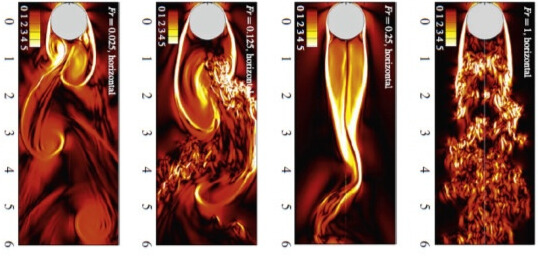
\includegraphics[width = 0.8\textwidth]{figures/fig_stokes/Stokes}
\caption*{Stokes flow around a circle with cyclic turbulence shedding.}
\end{figure}


\subsubsection{Chapter 8: Conclusion}


This chapter begins with the pursuit of a curiosity.  The question of whether a replication rate advantage, weighted towards the beginning of a branching process will lead it to generally outperform another process without the front weighting.  I should specify that a condition is imposed whereby the two compared models have overall the same "replicative potential".  In the case of discrete time branching, this condition manifests in the sum of the dividing probabilities being the same over a defined number of generations. \par 

\vspace{10pt}
\noindent
The reason for this curiosity was to determine whether there is some fundamental advantage to replication being weighted towards the outset.  It turns out not to be the case; there is no advantage (in the expected value at least), provided the condition. \par 

In the case of Y. pestis seeking a replicative advantage in host macrophages,  the condition of equivalent overall replicative potential of course doesn't hold.  Because taking the higher rate at the outset doesn't diminish the rate of extracellular replication. \par 
The next part of this chapters explores stochastic birth death style models which encorporate two phases.


\vspace{15pt}
\noindent
\textbf{Two phase models}
The first phase in each of the following models represents the pro-phagocytosis phase of Y. pestis pathogenesis.  The second phase represents extracellular growth. \par

A few versions are explored: 

\begin{itemize}
\item \textbf{Birth-death to birth-death}
With two successive birth death processes, the duration of the first can be controlled directly as a parameter.  And this indirectly controlls the initial count in the second phase.


\item \textbf{Birth-death-catastrophe to birth-death-catastrophe}
In the case of an initial BDC process followed by birth death, the duration of the first phase is determined indirectly by the bursting rate. 

\item \textbf{Constant to birth-death}
Here,  the initial count of the second phase is controlled directly. This is the same as what was described in part of the the Mathematical bacground section (demonstrating the importance of initial counts in slightly supercrictical birth death processes).  The closer to criticallity (from above) the process, the more significant the effect.  And it seems straightforward to argue (which I hope to do elsewhere) that most biological replication processes,  if they are supercritical at all, opperate close to the critical threshold. (This is of course excepting cases where the early stages of a logistic groth phase are still causing more substantially exponential growth). 


\item \textbf{Constatnt to birth-subdusive-death}  A subducive death rate simply means a death rate which declines as a function of time.  This assumption follows loosly from a theory that over time, Y. pestis will after progresing through more and more generation cycles, begin to adapt to the particular environment of that host.  The presence of host-symbiotic immuno bacteriophages could form the basis of an example in which this dynamic applies.  In other words, the first Y. pestis may not be able to subvert the attacks of certain present bacteriophages, but maybe its great grandaughter can.  \par 
If a dynamic like this were present, it could have the effect of causing the extracellular net-replication rate to begin sub-critical, and tend into supercriticallity over time. In this case, a larger initial cohort would be of vital importance,  this possibly being provided by the within macrophage phase. 
\end{itemize}


\noindent
\textbf{Quadrant argument}
There is a simple argument for why Y.  pestis would favour phagocytosis to begin with and an anti-phagocytosis strategy  when neutrophil recruitment takes place: That neutrophils are more effective killers,  and so Y. pestis would want to avoid them.  But why not resist phgocytosis to begin with? Likely because the macrophage intracellular environment permits some replicative advantage. This section mathematizes this straightforwad argument using the simple birth death process.


\FloatBarrier
\begingroup
\footnotesize
\bibliographystyle{unsrt}
\bibliography{references}
\endgroup

\end{document}
